\section{Simulation of Path Planner}

The same autopilot that was used for simulating the controller will be used when simulating the path planner. A path follower will be used to give course commands to the autopilot during simulation, while the rest of the states will be controlled only by the autopilot.


\subsection{Path Follower}
\label{ch:path_follower}

Two different path followers will be used in this simulation. The first path follower will be used to follow the Dubins path, while the second will be used to follow the continuous path that is generated as an improvement to the Dubins path.

The strategy used to follow Dubins path will be based on two algorithms presented in \cite{suaBEARD} by Beard \& McLain. The two algorithms are used to follow straight and curved line paths.

In order to follow straight line paths, the algorithm uses the position and heading of the aircraft, the previous waypoint and the direction from the previous to the next waypoint as input. The previous waypoint and direction to the next waypoint are given as output from the algorithm generating Dubins path described in chapter \ref{ch:dubins_path}. The new course is calculated so that the aircrafts position will converge towards the original path.

The algorithm for following circular paths is based on following perfect circles. Therefore it takes center and radius of the circle, the direction to orbit the circle, and the current position and heading of the aircraft. The heading calculated here will also ensure that the aircrafts position converges to the cirular path.

The altered path is based on the route that is flown in the first simulation, and will therefore not consist of circular arcs and straight lines. Instead the path will be a continuous path which requires a different path follower. The path follower will be based on the principles of Line Of Sight (LOS) steering laws presented by Fossen \cite{fartoyFOSSEN}.

Enclosure-based steering is LOS principle that considers a circle with radius $R$ enclosing the vehicle, which represents the LOS distance. Assuming that the radius is suffieciently large compared to the vehicle's distance from the path, the circle will intersect the path at two different points. One of the points will be in the direction of the vehicle, denoted $x_{los}$ and $y_{los}$. This is the point the vehicle will be directed to, and the course to that point can be expressed as \cite{fartoyFOSSEN}:

\begin{equation}
	\chi_d(t) = \text{atan2}(y_{los} - y(t), x_{los} - x(t))
\end{equation}

where $x(t)$ and $y(t)$ is the vehicle's current position. Using Pythagoras theorem, the points $x_{los}$ and $y_{los}$ can be found as:

\begin{equation}
	[x_{los} - x(t)]^2 + [y_{los} - y(t)]^2 = R^2
\end{equation}

where $R$ is the chosen LOS distance.


\subsection{Simulation Setup}

The simulation was performed using the same Simulink and Matlab setup as previously, using the path followers to generate the desired course angle. The Dubin's path that will be used as a reference is shown in figure \ref{fig:dubins_reference}.

\begin{figure}[!ht]
    \centering
    \makebox[\textwidth][c]{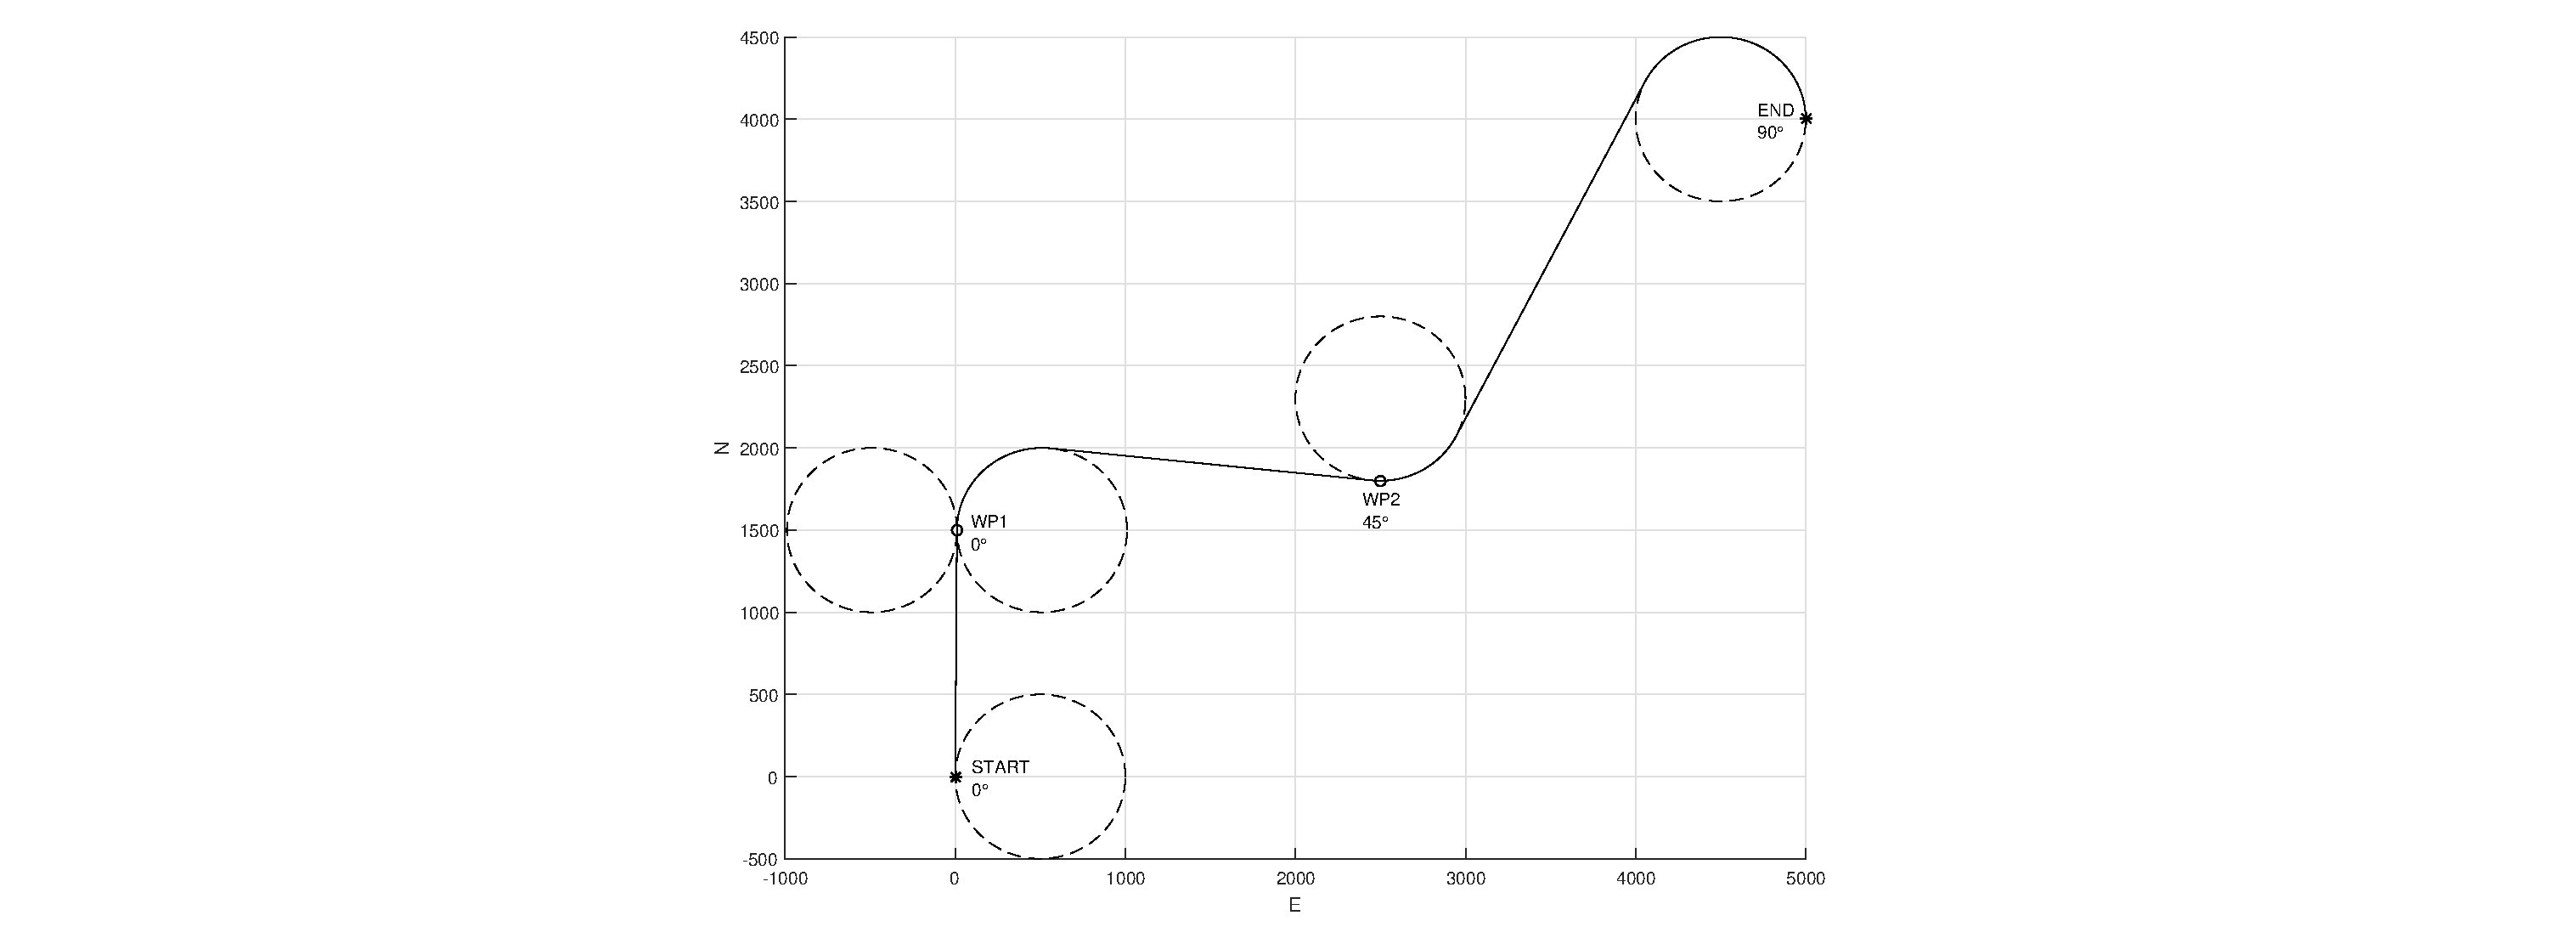
\includegraphics[width=2.2\textwidth, keepaspectratio=true]{dubins_reference.eps}}
    \caption{The path that will be simulated, with the direction associated with every waypoint.}
	\label{fig:dubins_reference}
\end{figure}

EXPLAIN WHY 600m RADIUS

\subsection{Results}